%%%%%%%%%%%%%%%%%%%%%%%%%%%%%%%%%%%%%%%%%%%%%%%%%%%%%%%%%%%%
%%  This Beamer template was created by Cameron Bracken.
%%  Anyone can freely use or modify it for any purpose
%%  without attribution.
%%
%%  Last Modified: January 9, 2009
%%

\documentclass[xcolor=x11names,compress]{beamer}

%% General document %%%%%%%%%%%%%%%%%%%%%%%%%%%%%%%%%%
\usepackage{graphicx}
%%%%%%%%%%%%%%%%%%%%%%%%%%%%%%%%%%%%%%%%%%%%%%%%%%%%%%

\usepackage[frenchb]{babel}

\usepackage[utf8]{inputenc}

\usepackage{lastpage}

\usepackage[round]{natbib}

\usepackage{caption}
\captionsetup{figurename=}

\usepackage{pgffor} \usepackage{fp} \usepackage{tikz}

\usepackage{appendixnumberbeamer} \usepackage{tikz}

%% Beamer Layout %%%%%%%%%%%%%%%%%%%%%%%%%%%%%%%%%%
\useoutertheme[subsection=false,shadow]{miniframes}
\useinnertheme{default} \usefonttheme{serif} \usepackage{palatino}

\setbeamerfont{title like}{shape=\scshape}
\setbeamerfont{title}{shape=\scshape}
\setbeamerfont{frametitle}{shape=\scshape}
\setbeamerfont{footline}{shape=\scshape}

\definecolor{MRed}{HTML}{8B0000} \definecolor{MGreen}{HTML}{008B00}
\definecolor{MBlue}{HTML}{00688B}

\setbeamercolor*{lower separation line head}{bg=MBlue}
\setbeamercolor*{normal text}{fg=black,bg=white}
\setbeamercolor*{alerted text}{fg=red} \setbeamercolor*{example
  text}{fg=black} \setbeamercolor*{structure}{fg=black}

\setbeamercolor*{palette tertiary}{fg=black,bg=black!10}
\setbeamercolor*{palette quaternary}{fg=black,bg=black!10}

\setbeamercolor{footlinerule}{bg=MBlue}
\setbeamercolor*{footlinecolor}{bg=black!10}

\setbeamercolor{block title}{use=structure,fg=white,bg=MBlue!75!black}
\setbeamercolor{block body}{use=structure,fg=black,bg=MBlue!20!white}

\setbeamercolor{block title
  example}{use=structure,fg=white,bg=MGreen!75!black}
\setbeamercolor{block body
  example}{use=structure,fg=black,bg=MGreen!20!white}

\setbeamercolor{block title
  alerted}{use=structure,fg=white,bg=MRed!75!black}
\setbeamercolor{block body
  alerted}{use=structure,fg=black,bg=MRed!20!white}

\renewcommand{\(}{\begin{columns}} \renewcommand{\)}{\end{columns}}
\newcommand{\<}[1]{\begin{column}{#1}} \renewcommand{\>}{\end{column}}
%%%%%%%%%%%%%%%%%%%%%%%%%%%%%%%%%%%%%%%%%%%%%%%%%%


\author{Arnaud Bletterer} \title{Outils multidimensionnels de
  déformation}

\newcommand{\mytext}{Outils multidimensionnels de déformation}

\graphicspath{{PresentationFigs/}}

%%%%%%%%%%%%%%%%%%%%%%%%%%%%%%%%%%%%%%%%%%%%%%%%%%%%%%
%%%%%%%%%%%%%%%%%%%%%%%%%%%%%%%%%%%%%%%%%%%%%%%%%%%%%%

\makeatother \setbeamertemplate{footline} {%
  \leavevmode
  \begin{beamercolorbox}[wd=\paperwidth,ht=1ex,dp=0ex,center]{footlinerule}
  \end{beamercolorbox}%

  % \hbox{\begin{beamercolorbox}[wd=1\paperwidth,ht=2.5ex,dp=1.125ex,leftskip=.3cm,rightskip=.3cm]{footlinecolor}%
  %   \count1 = \linewidth
  %   \divide\count1 by \inserttotalframenumber

  %   \foreach \n in {1,...,\insertpagenumber}{\hskip1.\count1}
  %   
\includegraphics[scale=0.06, viewport= 600 200 0 0]{cgogn}
   
  % \end{beamercolorbox}
  % }

  \hbox{\begin{beamercolorbox}[wd=.5\paperwidth,ht=2.5ex,dp=1.125ex,leftskip=.3cm,rightskip=.3cm]{footlinecolor}%
      \inserttitle
    \end{beamercolorbox}%

    \begin{beamercolorbox}[wd=.5\paperwidth,ht=2.5ex,dp=1.125ex,leftskip=.3cm,rightskip=.3cm]{footlinecolor}%
      \usebeamerfont{author in head/foot}\insertauthor\hfill
      \insertpagenumber /\inserttotalframenumber
    \end{beamercolorbox}}%
  \vskip0pt%
} \makeatletter

%%%%%%%%%%%%%%%%%%%%%%%%%%%%%%%%%%%%%%%%%%%%%%%%%%%%%%
%%%%%%%%%%%%%%%%%%%%%%%%%%%%%%%%%%%%%%%%%%%%%%%%%%%%%%

\begin{document}

%%%%%%%%%%%%%%%%%%%%%%%%%%%%%%%%%%%%%%%%%%%%%%%%%%%%%%
%%%%%%%%%%%%%%%%%%%%%%%%%%%%%%%%%%%%%%%%%%%%%%%%%%%%%%
\section{\scshape Introduction}
\begin{frame}
  \title{Outils multidimensionnels de déformation\\~\\

    \begin{figure}
      \begin{center}
        
\includegraphics[scale=0.3]{uds-logo}~~~~~~~~~
        
\includegraphics[scale=0.15]{icube-logo}
      \end{center}
    \end{figure}
  }
  \author{Arnaud Bletterer \\
    \textit{Université de Strasbourg} \vspace{-0.5cm}\date{\today} } \titlepage
\end{frame}

%%%%%%%%%%%%%%%%%%%%%%%%%%%%%%%%%%%%%%%%%%%%%%%%%%%%%%
%%%%%%%%%%%%%%%%%%%%%%%%%%%%%%%%%%%%%%%%%%%%%%%%%%%%%%
\begin{frame}{Sommaire}
  \tableofcontents
\end{frame}

%%%%%%%%%%%%%%%%%%%%%%%%%%%%%%%%%%%%%%%%%%%%%%%%%%%%%%
%%%%%%%%%%%%%%%%%%%%%%%%%%%%%%%%%%%%%%%%%%%%%%%%%%%%%%
\section{\scshape Etat de l'art}
\subsection{Introduction}

\begin{frame}{Contexte}
  Déformation spatiale
  \begin{itemize}
  \item Indépendant de la représentation interne
  \item Manipulation à l'aide d'un outil
    \begin{itemize}
    \item Discrétisé en cellules (point, courbe, surface, volume)
    \item Manipulation directe des points de contrôle
    \item Différentes caractéristiques (résolution, zone d'influence)
    \end{itemize}
  \end{itemize}
\end{frame}

\begin{frame}{Introduction}
  \begin{itemize}
  \item Création d'un outil multidimensionnel
  \item De manière automatique
  \item Et paramétrable
  \end{itemize}
\end{frame}

\begin{frame}{Création d'un outil multidimensionnel}
  \begin{block}{Mélanger plusieurs outils}
    \begin{itemize}
    \item Différentes dimensions/résolutions
    \item Déformation lisse (au moins $C^1$)
    \end{itemize}
  \end{block}
  \begin{alertblock}{Problèmes}
    \setbeamercolor{itemize item}{fg=MRed}
    \begin{itemize}
    \item Finesse de la déformation liée au nombre de DDL
    \item Comment faire communiquer les différents outils?
    \end{itemize}
  \end{alertblock}
  \begin{figure}[h]
    \begin{center}
      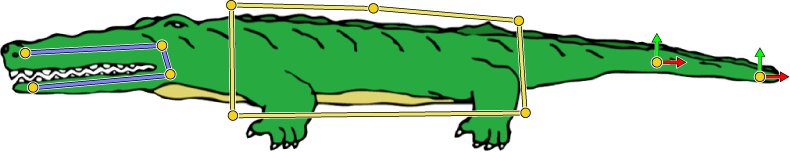
\includegraphics[scale=0.15]{alligator-avant.png}
      
\includegraphics[scale=0.15]{alligator-apres.png}
    \end{center}
    \caption{Image de \cite{JBPS11}}
  \end{figure}
\end{frame}

\begin{frame}{De manière automatique}
  \begin{block}{Associer les outils adaptés}
    \begin{itemize}
    \item Découper un modèle
    \item
    \end{itemize}
  \end{block}
\end{frame}


%%%%%%%%%%%%%%%%%%%%%%%%%%%%%%%%%%%%%%%%%%%%%%%%%%%%%%
%%%%%%%%%%%%%%%%%%%%%%%%%%%%%%%%%%%%%%%%%%%%%%%%%%%%%%
\section{\scshape Méthode implémentée}
\subsection{frame}
\begin{frame}{frame}

\end{frame}

%%%%%%%%%%%%%%%%%%%%%%%%%%%%%%%%%%%%%%%%%%%%%%%%%%%%%%
%%%%%%%%%%%%%%%%%%%%%%%%%%%%%%%%%%%%%%%%%%%%%%%%%%%%%%
\section{\scshape Continuité}
\begin{frame}{Continuité}

\end{frame}

\appendix

\begin{frame}<beamer:0>
\bibliographystyle{plainnat}
\bibliography{../Rapport/References/references.bib}
\end{frame}


\end{document}